\documentclass[11pt]{article}

\usepackage[margin=1in]{geometry}
\usepackage{amsmath}
\usepackage{booktabs}
\usepackage{graphicx}
\usepackage[numbers,square]{natbib}
\usepackage[colorlinks=true,linkcolor=blue,citecolor=blue,urlcolor=blue]{hyperref}

\setlength{\emergencystretch}{2em}
\newcommand{\ngvla}{ngVLA}
\newcommand{\arcsec}{^{\prime\prime}}

\title{An ngVLA Science Subarray Selection Heuristic}
\author{Brian Mason, Michael Stroh}
\date{23 September 2026 (v1)}

\begin{document}
\maketitle

\begin{abstract}
  We describe a heuristic for choosing an \ngvla\ reference
  subarray and the {\tt tclean} visibility weighting parameters that
  meet a given set of quantitative science requirements (angular
  resolution, largest angular scale, sensitivity, and PSF-quality)
  while minimizing either antenna-hours or integration time on source.
  Using a set of noise-only CASA simulations at 30 GHz, the method
  pre-tabulates for each subarray the achieved resolution and
  sensitivity penalty $\eta$ for the selected visibility weighting
  (relative to natural weights)--- as well near-in PSF sidelobe
  (``skirt'')--- over a lattice of robust and taper values. We also
  describe prototype implementations of this heuristic as a web calculator
  and a python module.
\end{abstract}

\section{Introduction}
\label{sec:intro}

In order to address a diverse range of science projects, currently
anticipated and yet to be imagined, the Next Generation Very Large
Array (\ngvla) has antennas configured so as to provide images at a
wide variety of angular resolutions on the sky
\citep{configDescription,memo106}.  In order to minimize construction
and operations cost--- thereby ultimately freeing resources to enhance
fundamental observing capabilities such as collecting area--- the
design does not include movable antennas.  Instead, the locations of
the antennas are chosen so as to support the full range of \ngvla\
science observations flexibly.  The vast majority of these
observations will require only a subset of the antennas, also known as
a subarray.  In order to maximize the science throughput of the
\ngvla, it will typically--- perhaps, effectively, always--- be
operated with multiple subarrays observing commensally, in parallel.

A high-level concept for how this operation could work is presented in
\citep{saNarrative}.  Key aspects of this concept for our purposes
are:
\begin{enumerate}
\item A set of roughly two dozen ``reference subarrays'', which are
  pre-defined (in operations, with some flexibility).  These consist
  of individual array ``components'' (e.g.\ spiral, core, mid);
  combinations of these components (e.g.\ spiral+core, mid+spiral);
  and complementary combinations of subsets of them (e.g.\
  spiral+outer half core, inner half core).
\item A subarray (SA) recommendation engine for the Proposal
  Submission Tool (PST), which Principal Investigators (PIs) can use
  to get a ranked list of recommended subarrays that can achieve their
  science goals, expressed as broad but quantitative metrics like
  angular resolution, largest angular scale, and desired sensitivity.
  This is the functionality described in this memo.
\item Observing allocations based on equivalent time in a designated reference
  subarray (nominally: the top-ranked reference SA from the recommendation
  engine).
\item The capability in operations to re-assign a given
  observation's reference subarray at any point from proposal
  selection and time allocation to the collection of the first data
  from a given scheduling block (SB).  This capability will be
  essential to reduce observing pressure and provide operational
  flexibility.  The reference subarray a given SB ends up assigned to
  at the point of the first observation is called the ``assigned
  subarray''.
\item Some (bounded) flexibility in the actual SA(s) used for
  observation, relative to the assigned reference subarray.
\item A mechanism to ensure that SA re-assignments are fair, in the
  sense of still supporting the PI's science.  This mechanism would
  most likely use similar (or identical) heuristics as the SA ranking
  engine in the PST.
\end{enumerate}
Considerable complexity and technical risk exists in the closely
related processes of scheduling, and automated imaging of the
resulting data across a diverse range of science cases (discussed
below).  The relatively conservative approach to subarraying
recommended in \citep{saNarrative} is intended to provide a tractable
path--- for prototyping and eventual implementation--- to retiring
some of the technical risk in the intertwined problems of SA
assignment, scheduling, and pipeline imaging.

One challenge in SA assignment (and re-assignment) arises from the
\ngvla's hierarchical, multi-angular-scale array configuration.  In
the context of the currently prevailing algorithm used to make images
out of data from interferometers\footnote{Clean
\citep[e.g.][]{hogbom,clark, schwab}, or {\tt tclean} to use the name
of the task that implements Clean in CASA.}, the point-spread
functions (PSFs) of such configurations can give rise to instabilities
in the deconvolution process.  The naturally weighted PSF of the main
array, for example, has a broad skirt, well beyond the fitted Gaussian
core of the beam, at more than half the peak level
\citep{memo65,memo121}.  To reliably eliminate these instabilities, it
has so far been recommended \citep{memo65,memo72,memo76,memo106} to
use Briggs robust weighting \citep{briggs}, often with $r < 0$,
sacrificing considerable sensitivity in the process.  Under this
approach different subarrays end up with different sensitivity
penalties at a given angular resolution, which needs to be accounted
for in SA assignment and re-assignment.  \citep{memo121} did this for
the Envelope Observing Program (EOP) using a considerably larger set
of simulations (see \S\ref{sec:sims} for discussion).

The purpose of the present memo is to describe a heuristic--- and its
prototype implementation--- that performs this task automatically and
in a way suitable for use as a general purpose calculator in the
context of the ngVLA Subarray Concept \citep{saNarrative}. The heuristic's
inputs are specific, mostly quantitative parameters describing the
primary science intent of the observation. Its outputs are
a list of subarrays, estimated observing times, and imaging parameters (under
an assumed imaging scenario), rank-ordered by a selectable creterion.

\section{Methodology}
\label{sec:method}

\subsection{Science Intent}
\label{sec:scienceIntent}

The PI science intent is represented by: a desired sensitivity (in
either flux density per beam or Kelvin units) $\sigma_0$; a velocity
channel width $\delta v$ (continuum over the full receiver bandwidth
if omitted); a desired angular resolution $\theta_{\rm req}$; a
desired largest angular scale to recover, $\theta_{\rm LAS,req}$; and
an observing frequency $f$ within the \ngvla\ range.  Angular
resolution is understood throughout as the geometric mean of the
major and minor axes of the fitted Gaussian restoring beam.

Additionally, the PI specifies whether PSF quality is a constraint on
SA selection and ranking (observation type ``imaging'') or is not
(observation type ``point source'').  For imaging observations, the
maximum allowed PSF ``skirt'' level is specifiable (the python
interface accepts any value; the web calculator accepts 5\%, 10\%,
15\%, or 20\%).  The skirt is defined, following \citep{memo106}, as
the azimuthally averaged PSF level at a radius of one fitted FWHM from
the peak, expressed as a fraction of the PSF peak.  Note that a purely
Gaussian beam has a skirt of $\sim 6\%$ by this definition, so 5\% is
a stringent choice and 10\% (the memo 121 default, originally
suggested in \ngvla\ memo 47) permits a modest departure from
Gaussianity.  This quantity is the primary proxy for PSF quality, and
the only one (besides FWHM) used in subarray selection and ranking.

Finally, the PI (or the observatory) states whether the ranking should
minimize integration time or antenna hours, and the fractional
tolerance $\delta \theta$ on the achieved beam (default 5\%). Two
legacy ranking modes are also supported. For more details on these
see \S~\ref{sec:selection}.

\subsection{Reference Subarrays}
\label{sec:refsa}

Table~\ref{tab:subarrays} lists the Rev.\,F reference subarrays
currently tabulated.  The first seven (core-inner through main) are
the components and simple combinations; the remaining seven are the
LONG-bearing and outer-core combinations introduced by
\citep{memo121}.  Core-outer is the outer 57 core antennas by radius
(the ``outer50core'' of memo 121); it is not offered on its
own\footnote{One further combination, core+mid, was accidentally
simulated by Claude. It is not a useful configuration.}.  This is
about half the set of $\sim 24$ reference subarrays envisaged in
\citep{saNarrative}; the SBA and total-power array have not yet been
considered.

Some heterogeneous subarrays--- i.e. some of the SAs combining
distinct array components measuring different angular scales, such as
mid+long--- have caps imposed on the offered resolution
range. Specifically main, mid+long, main+long, spiral+mid+long and the
three core-outer combinations (spiral+core-outer,
mid+spiral+core-outer, long+mid+spiral+core-outer), have the coarsest
resolution offered capped at the native beam of the next-to-largest
component subarray: core for main, core-outer for the core-outer
combinations, mid for mid+long, main for main+long, and spiral+mid for
spiral+mid+long.


\begin{table}[tb]
\centering
\small
\caption{Rev.\,F reference subarrays tabulated in the prototype.
  $N$ is the number of 18m antennas; $b_{\min}$ and $b_{\max}$ are
  the shortest and longest baselines after the LONG short-baseline
  filter, where applied; LAS is $0.8\,\lambda/b_{\min}$ at 30 GHz
  (\S~\ref{sec:heuristic}); the beam cap is the coarsest resolution
  offered at 30 GHz for heterogeneous subarrays (blank where the only
  limit is the $20\times$ natural-beam end of the taper lattice).
  $b_{\min}$ for main+long is unfiltered (\S~\ref{sec:sims}).}
\label{tab:subarrays}
\begin{tabular}{@{}lrrrrr@{}}
\toprule
Subarray & $N$ & $b_{\min}$ (m) & $b_{\max}$ (km) & LAS ($\arcsec$) & Beam cap ($\arcsec$) \\
\midrule
core-inner                 &  57 &    42.2 &     1.63 & 39.3   & --      \\
core                       & 114 &    42.2 &     4.27 & 39.3   & --      \\
spiral                     &  54 &   811.4 &    39.3  & 2.04   & --      \\
mid                        &  46 & 10121   &  1273    & 0.163  & --      \\
core+spiral                & 168 &    42.2 &    39.3  & 39.3   & --      \\
spiral+mid                 & 100 &   811.4 &  1273    & 2.04   & --      \\
main (core+spiral+mid)     & 214 &    42.2 &  1273    & 39.3   & 0.710   \\
long                       &  30 & 515162  &  8686    & 0.0032 & --      \\
mid+long                   &  76 & 10121   &  8686    & 0.163  & 0.00296 \\
spiral+mid+long            & 130 &   811.4 &  8686    & 2.04   & 0.0111  \\
main+long                  & 244 &    36.7 &  8686    & 45.1   & 0.0212  \\
spiral+core-outer          & 111 &   179.0 &    39.3  & 9.25   & 0.491   \\
mid+spiral+core-outer      & 157 &   179.0 &  1273    & 9.25   & 0.491   \\
long+mid+spiral+core-outer & 187 &   179.0 &  8686    & 9.25   & 0.491   \\
\bottomrule
\end{tabular}
\end{table}

\subsection{Simulations}
\label{sec:sims}

A fixed suite of simulated measurement sets--- one per reference
subarray--- is generated in CASA.  All of the simulations are done at
30 GHz, with: a single pointing, one 1 MHz channel, 60 second
integrations, a four hour track (hour angle $\pm 2$ h) on a source at
declination $+24^\circ$, and thermal noise only (no sky model).  The
MS is corrupted with a single realization of Gaussian noise using the
default seed, from which the dirty-image rms is measured
directly. Once generated, the MS is kept on disk for later
use (on TACC, the MS's are kept on {\tt \$WORK}).

The simulation running infrastructure and the calculators both support
the capability of tabulating results for different antenna
configurations and observing and imaging modes. These different sets
of simulations, corresponding to different antenna configurations and
observation parameters, are called ``campaigns''.  The released
calculator has three campaigns: single-channel, 4-hour tracks with
each of Rev-F, Rev-D, and Rev-C. Rev-F has the most refined set of
simulations. It could also be considered to run snapshot and/or MFS
campaigns (see discussion in \S~\ref{sec:discussion}), and there is
some code in place, but it is not yet well validated.

\subsection{Imaging Sweeps and Refinement}
\label{sec:img}

Images are made with {\tt tclean} at a fixed imsize in pixels for each
subarray: 4096 for most single-component subarrays (core, spiral,
mid); 8192 for core+spiral, spiral+mid, and long; and 15000 for main,
mid+long, and spiral+mid+long. The cell size is the
maximum\footnote{The choice (made by Claude based on an option in the
pre-existing taper-ability pipeline) to grow the image with uv-taper
is debatable. It's likely not consequential for the intended
applications, but could be fixed in a future version.} of the native
cell size and the uv-taper/5, where the native cell size is the pixel
size implied by the longest baseline, given by {\tt im.advise()}. The
resulting images are all larger than $245^2$ beams in size
(fitted/actual beams, not native cell $\times 5$); typically they are
$400^2$ to $600^2$, with long and mid+long at $\sim 1250^2$.  These
choices trade adequate noise statistics and sampling of the PSF
plateau--- both of which prefer larger images--- against compute
cost and the effectiveness of $uv$-weighting, both of which prefer
smaller images. This is discussed more in \S~\ref{sec:discussion}.

The LONG component contains small groups of $\sim 3$ antennas with
$\sim 37$--$176$~m spacings, in addition to its multi-thousand-km
baselines.  These short baselines are irrelevant to imaging with LONG
and would distort its PSF, so visibilities with $\sqrt{u^2 + v^2}
\lambda < 178$~m are excluded before imaging from subarrays containing
LONG, except main+long, whose core supplies legitimate baselines below
that length\footnote{The $36.7$~m minimum in Table~\ref{tab:subarrays}
is one of the intra-LONG-station baselines; both HP and HN have
baselines of about this length.}.

For each desired lattice point a dirty, noise-only image and PSF are
made.  We record the restoring beam fitted by {\tt tclean} to the main
lobe of the PSF (major and minor FWHM and position angle), and take
the geometric mean of the two axes as the resolution $\theta$; the
dirty-image rms, which gives $\eta$ once normalized by the RMS of the
natural, untapered point; and the azimuthally averaged PSF out to a
radius of 10 (CASA-fitted) FWHM. The PSF skirt $s$ is measured from
the radial profile, defined following \citep{memo65} as the
azimuthally averaged PSF level at a radius of one fitted FWHM from the
peak, using annular means one cell wide interpolated with a cubic
spline. We also calculate and record, from the azimuthally averaged
PSF\footnote{The beam volume calculated this way is exact. The volume
of the beam-squared calculated this way is a slight under-estimate.},
the half-power width; the volume of the PSF out to its first null or
inflection; and the volume of the PSF-squared out to its first null or
inflection. These are generally useful PSF diagnostics; the
beam-squared is used for the confusion calculation. Where the profile
has no zero crossing--- common for the two-scale composite
subarrays--- the first resolved minimum is used.  On TACC, the imaging
run byproducts go to {\tt \$SCRATCH}, where they are periodically
purged.

Initially the PSF characteristics and $\eta$ are calculated from the
simulations on an {\it a priori} grid in robust and taper $(r,t)$:
natural weighting and Briggs robust from $-2$ to $+2$ in steps of 0.4,
each crossed with no taper plus 14 (18 for heterogeneous subarrays)
logarithmically spaced tapers spanning $0.3\times$ the $r=-2$ beam to
$20\times$ the natural beam.  The resulting curves
(\S~\ref{sec:heuristic}) are then automatedly inspected for holes,
jumps, and non-monotonic stretches in resolution. Where bilinear
interpolation between measured points is not a good predictor of an
intermediate point's value, additional $(r,t)$ points are imaged from
the existing simulations.  This refinement was repeated for several
rounds until most of the simulation points validate and the curves
look reasonable; the final tables have between $\sim 250$ and
$\sim 700$ points per subarray.

The strategy used here results in one simulated MS per subarray, which
is then imaged many times depending on how many $(r,t)$ samples are
needed in the end to construct an adequate performance curve. Previous
beam sculpting work (\cite{memo121} and references therein) performed
one simulation for each science case, times however many subarrays
were considered for that science case.  In Memo 121, for example,
three subarrays were considered for each science case: Main, plus the
``efficient'' and ``performance'' subarrays, as defined there. In both
cases the $N_{images}$ axis multiples this, but here all imaging runs
are useful for any run using the SA in question.  By simplifying the
simulation infrastructure to a single reference frequency (30 GHz),
the approach used here enables construction of a general purpose
tool. It also more straightforwardly supports considering a wider
range of subarrays for a given science case, enabling producing
multiple viable options in many cases (i.e. the ranked list).


\section{Science Subarray Selection Heuristic}
\label{sec:heuristic}

The science subarray assignment and ranking works, at a high level, as
follows.  For each reference subarray $i$ we have (input/meta-data)
values $(N_i, b_{\min,i}, C_{{\rm LAS},i}, \theta_{{\rm cap},i})$,
where $N_i$ is the number of antennas in the subarray; $b_{\min,i}$
the shortest baseline; $C_{{\rm LAS},i}$ the factor assumed to relate
the shortest baseline to the LAS, so that $\theta_{{\rm LAS},i} =
C_{{\rm LAS},i}\,\lambda/b_{\min,i}$; and $\theta_{{\rm cap},i}$ the
coarsest resolution offered (at 30 GHz) for the subarray in question.
We adopt $C_{\rm LAS}=0.8$ for all subarrays, comparable to the value
$0.85$ found in \citep{memo67}; \citep{memo67} found $\sim 0.6$ for
the SBA.  We also assume that the LAS is independent of $r$ and $t$.
Both assumptions could fairly straightforwardly be checked.

As described in \S~\ref{sec:sims}, there is a simulated MS for each
subarray, from which the imaging performance characteristics---
resolution $\theta$, noise penalty $\eta$, and PSF skirt height $s$---
have been measured for a collection of robust and taper values.  A
given lattice point $(r,t)$ is called $p$.  The noise penalty for a
given subarray is defined, following \citep{memo55} and
\citep{memo121}, as
\begin{equation}
  \eta(p) = \frac{\sigma_{\rm dirty}(p)}{\sigma_{\rm dirty}({\rm natural},\,t=0)} ,
\end{equation}
i.e.\ the dirty-image rms at $p$ normalized to the natural,
untapered rms of the same subarray.\footnote{The natural points are
explicitly simulated and measured, not taken from $r=2$.}  Natural
weighting has $\eta = 1$ by construction and is the
sensitivity-optimal point; every other choice of $(r,t)$ has
$\eta \ge 1$ up to the measurement scatter of a single noise
realization.  Because $\eta$ is a ratio of rms values for the same
subarray, the corresponding integration time to reach a fixed
point-source sensitivity scales as $\eta^2$, and the antenna hours as
$N_i\,\eta^2$.

The subarray selection heuristic itself then selects those subarrays
from the set that provide the requested angular resolution and LAS.
The resulting set of subarrays are then ranked using $\eta$ and, if
PSF quality is of interest, by $s$. This process is described in
more detail in \S~\ref{sec:curvegen} and \S~\ref{sec:selection}.


\subsection{Curve Generation}
\label{sec:curvegen}

For visual presentation, and to create a more portable and legible
product, the set of several hundred simulation results for each
subarray is used to infer a small number of one-dimensional
performance curves: one point source curve, $\eta(\theta)$ and one imaging curve for
each skirt threshold $\eta(\theta;s_0)$.  Each curve gives the optimal $\eta$ as a
function of resolution $\theta$ under some condition:
\begin{itemize}
\item the {\it point-source} curve returns the $(r,t)$
  that gives the lowest $\eta$ subject to the constraint
  that $\theta_{req}/(1+\delta \theta) < \theta < \theta_{req} \times (1+\delta \theta)$, with
  no constraint on PSF shape ($s$).
  This is the the taperability curve
  in the sense of \citep{memo55} and \citep{memo72}; and
\item the {\it imaging} curve 
  $\eta_{\rm im}(\theta; s_0)$ returns the point $(r,t)_i$ that
  minimizes $\eta$ subject to the constraints: $s < s_0$ and 
$ \theta_{req}/(1+\delta \theta) < \theta_i <  \theta_{req} \times (1+\delta \theta)$.
  If there are no points in the desired resolution range with $s < s_0$,  
  the point is returned that minimizes $s$ and
  it is marked as ``relaxed''.  
\end{itemize}
The minima are taken over the measured lattice points and bi-linearly
within each cell defined by four points $p$. $\eta$ and $t$ are
interpolated in the logarithm, and $s$ linearly in $\log\theta$.  The
engine does not extrapolate beyond the ends of a measured row, so a
gap in the sweep appears as a gap in the curve.

Note that $\eta_{\rm im} \ge \eta_{\rm ps}$ everywhere, and the two
curves coincide wherever the sensitivity-optimal weighting already has
an acceptable skirt. Note also that the logic of the dual-parameter
optimization described above can sometimes give rise to bifurcations
that appear as steps in the  $\eta(\theta;s_0)$ curve, where the $s_0$
request is satisfiable on one side but not the other.

\subsection{Selection and ranking}
\label{sec:selection}

Given a PI's request $R = (\sigma_0, \delta\nu, f, \theta_{\rm req},
\theta_{\rm LAS,req}, {\rm type}, s_0)$ the calculator proceeds as
follows for each reference subarray $i$:
\begin{enumerate}
\item Scale the request to the 30 GHz reference frame, $\theta_{\rm
  req}^{(30)} = \theta_{\rm req}\,(f/30\,{\rm GHz})$, and likewise
  $\theta_{\rm LAS,req}$.  This assumes that $\eta$ and $s$ at a given
  $(r,t)$, expressed in units of the native beam, are independent of
  frequency; this is exact for the $uv$ coverage of a single channel.
  It would be approximate for (MFS) continuum imaging with varying
  fractional bandwidths between bands.
\item Exclude the subarray if the tolerance window about
  $\theta_{\rm req}^{(30)}$ lies entirely outside the range spanned by
  its curve (finer than the finest tabulated beam, or coarser than
  $\theta_{{\rm cap},i}$).
\item If an LAS was specified, exclude the SA in question if
  $\theta_{{\rm  LAS},i} < \theta_{\rm LAS,req}$.
\item Identify the optimum lattice or curve point for the selected
  mode, imaging or point source, by the logic of \S~\ref{sec:curvegen}.
  Note that at present, the python calculator uses a look-up table
  with all measured lattice points; the web calculator uses the
  curves constructed as described in \S~\ref{sec:curvegen}.
\item Scale the taper $t$ back to the requested frequency.
\item Compute the integration time $\tau_i$ needed to reach $\sigma_0$
  in a channel of width $\delta\nu$ at $\theta_{\rm req}$ with $N_i$
  antennas and rms penalty $\eta_i$, using the python implementation
  of the \ngvla\ sensitivity
  calculator\footnote{\url{https://gitlab.nrao.edu/vrosero/ngvla-sensitivity-calculator}},
  which incorporates the $T'_{\rm sys}$ model of \citep{memo96}; and
  the antenna hours $N_i\,\tau_i$.  If no sensitivity was requested, a
  fiducial goal (the one-minute natural-weighting rms of the main
  array at $f$) is used so that the ranking is still defined.
\end{enumerate}

For point-source mode requests, candidate SAs that meet the resolution
and LAS criteria are ranked by the chosen ranking criterion and
presented in a single tranche.  For imaging-mode requests, two
tranches of subarrays are returned: the first comprising those (if
any) that met the skirt-level request, and the second those that did
not. Each tranche is sorted internally by the selected ranking
criterion. For either mode, rejected SAs are also returned in a second
(or third) tranche which is not rank-ordered internally.

There are currently four ranking methods, two primary methods and two
legacy methods based on those used in \cite{memo121}:
\begin{enumerate}
\item {\it Antenna hours}: rank SAs by $\tau_i N_i$, smallest first.
  This is the default ranking method since antenna hours is the
  natural metric of a set of commensally operated subarrays.
\item {\it Integration time}: rank SAs by $\tau_i$ smallest first.
  This method minimizes the observing time needed for each individual
  observation. It would be appropriate to maximize the chances
  of success for highly-ranked individual observations that require
  rare weather conditions, as suggested by \cite{saNarrative}.
\item {\it Baseline efficiency}: rank SAs, largest first, by the
  fraction of its baselines falling within the range of baselines
  required. The largest baseline required is defined by treating the
  requested resolution as arising from an Airy disk of diameter
  $b_{max} = 1.02 \lambda/\theta_{req}$.  The shortest baseline
  required is defined as in \S~\ref{sec:heuristic}.  If an LAS is not
  specified, $b_{min}$ is imputed as that which would be required to
  achieve an $LAS = \theta_{req} \times 10$, although that LAS is not
  used for any other purpose (e.g., excluding SA's).
\item {\it Baseline performance}: rank SAs, largest first, by the {\it
  number of total baselines} falling within the range of baselines
  required. The same $b_{min}$ logic is used as for the ``efficient''
  ranking heuristic. We do not manually exclude Main as was done in
  \cite{memo121}, since this is not necessary when returning the full
  ranked list of candidates; it does often naturally occur as the
  first SA under this criterion.
\end{enumerate}
The legacy (``efficient'' and ``performance'') rankings do not
explicitly account for variations in $\eta$ between SAs, although the
given observing time estimates do account for $\eta$; whether this is
an advantage or a disavantage depends on whether the robust and taper
weighting is used to make the science images
(\S~\ref{sec:discussion}).  We chose to define $b_{max}$ with
reference to fundamental, subarray-independent concepts in contrast to
\cite{memo121}, which used a lookup table to define an effective
$b_{max}$ for each SA based on its naturally weighted beam. We also
added the $b_{min}$ guardrail described above to cover the case where
no LAS was specified, in order to avoid giving preference to SAs with
many short baselines for observations that do not need to constrain
large spatial scales. As stated above this imputed $b_{min}$ is not
used for excluding SAs, only for ranking them if the efficient or
performance ranking heuristic was chosen.

A ranked list of all reference subarrays is always returned, as
described above.  Each SA has metadata clearly indicating which
tranche it belongs to, and if it is in the tranche of failures, what
the reason(s) for failure were.

\subsection{Prototype Web and Python Subarray Calculators}
\label{sec:code}

Two prototype subarray calculators implementing the heuristics
described in this memo have been produced: a python calculator, and a
web (html+javascript) calculator.  A high-level architecture diagram of how these
applications relate to the suite of simulations behind them is in
Fig.~\ref{fig:arch}.

The web calculator is maintained at
\url{http://www.cv.nrao.edu/~bmason/ngvla-curves-release.html}.
The code, including the python calculator, are at
\url{https://github.com/bmason72/ngvla_subarrays}

In addition to ranking subarrays, the calculators provide:
\begin{itemize}
\item The volume of the achieved PSF out to the first null or inflection point,
  divided by the fitted clean beam volume;
\item An estimate of the confusion, using the approximate area of the achieved
  beam-squared plus, the observing frequency, and the confusion model used by
  the sensitivity calculator \citep{condon2012,matthews2021};
\item  The number of visibilities {\it per channel} that will be generated
  by an observation of the needed duration for each subarray with 10-second dump times.
\end{itemize}

A couple of key differences between the web and python calculators are:
\begin{itemize}
\item The python calculator directly calls the python version of the
  ngVLA sensitivity calcaultor. The web calculator has a pretabulated
  natural-weight point source sensitivity for each subarray at a grid
  of frequencies assuming 1 MHz channel width; and a pre-tabulated
  confusion model.
\item The python calculator has all measured lattice points. The web
  calculator has these collapsed down into the curves described
  in \S~\ref{sec:curvegen}.
\end{itemize}

The python and html/javascript code were written almost entirely by a
combination of Claude Code (mostly) and Codex (when Claude tokens were
low, and for a complementary perspective) running at TACC. It
implemented and routinely performed an extensive test suite with $\sim
260$ unit tests, $\sim 190$ end-to-end/regression tests, and several
dozen other tests (e.g.  data contract tests). Validation of the
results was done by the authors periodically, and at the end.

\begin{figure}[tbp]
\centering
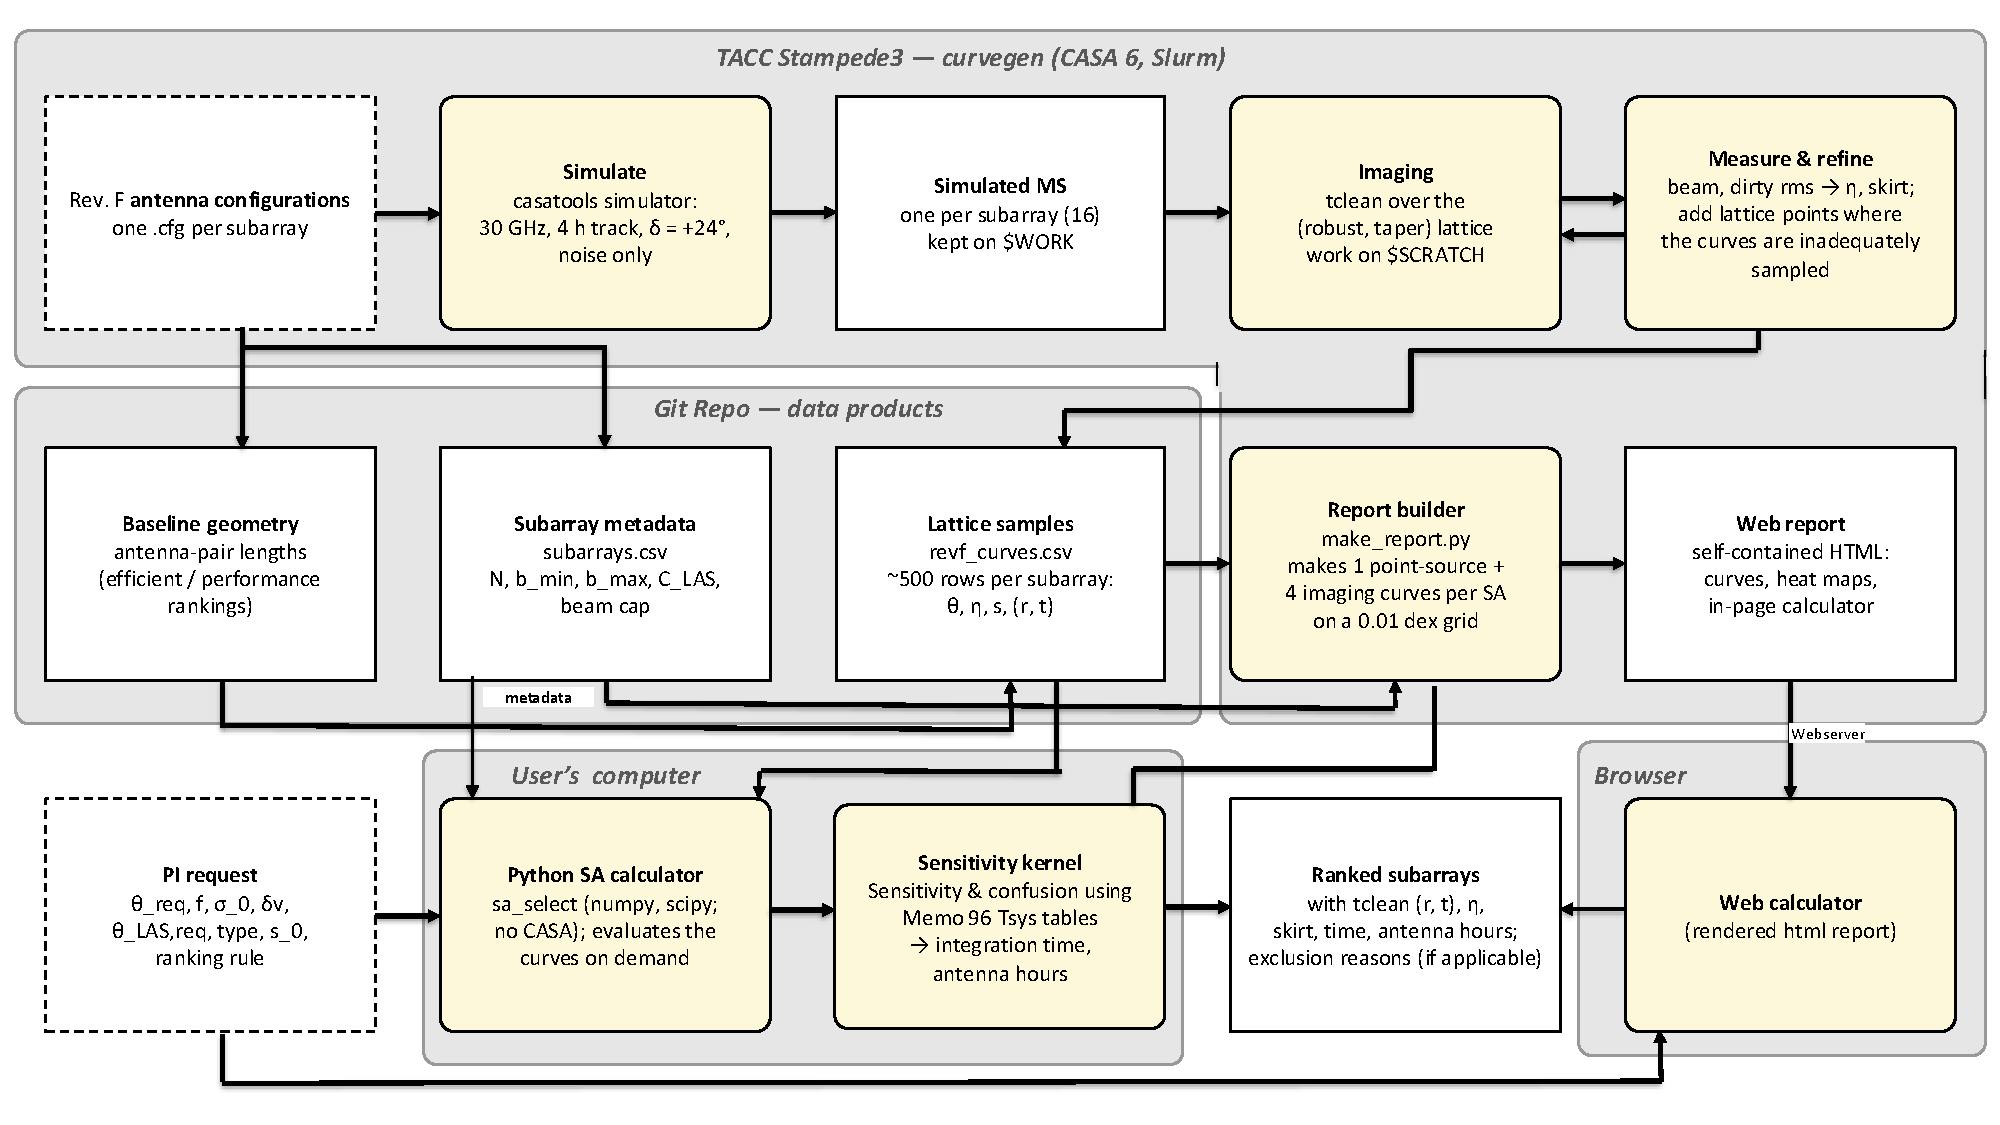
\includegraphics[width=\linewidth]{figs/architectureRefined.pdf}
\caption{High-level architecture of the prototype ngVLA subarray calculator.
  {\bf Square, white boxes} represent data, with {\bf dashed} boundaries
  denoting inputs and {\bf solid} boundaries denoting output products (intermediate or final).
 {\bf Rounded, yellow boxes} represent a process operating on the data.}
\label{fig:arch}
\end{figure}


\section{Rev.\,F Subarray Performance Curves}
\label{sec:curves}

Figures~\ref{fig:taper} and \ref{fig:imaging} show the point-source
and imaging ($s_0=10\%$) curves for the fourteen subarrays of
Table~\ref{tab:subarrays}, at 30 GHz.  Several features are worth
pointing out.
\begin{itemize}
\item The single components (core-inner, core, spiral, mid, long) meet
  the 10\% skirt criterion at every tabulated resolution, though the
  LONG-containing subarrays often have other strong PSF features.
  Their natural skirts are already 9\%--23\%, so the imaging curve
  lies within $\sim 10$--$30\%$ of the point-source curve near the
  native beam and coincides with it once the taper dominates.
\item The composites containing LONG (mid+long, spiral+mid+long,
  main+long, long+mid+spiral+core-outer), and also
  mid+spiral+core-outer, do not
  reach a 10\% skirt anywhere in their offered resolution range with
  robust weighting and taper alone; the best achievable skirt is
  mostly in the 10\%--25\% range, and exceeds 25\% at the finest
  resolutions, near LONG's own native beam.  For these subarrays the
  imaging curve consists entirely of relaxed points.  
\item The intermediate composites (core+spiral, spiral+mid,
  spiral+core-outer) meet the threshold over part of their range and
  are relaxed, but never worse than 25\%, over the rest.  The main
  array (natural skirt 57\%) is relaxed over nearly all of its range;
  this is the case that motivated beam sculpting in the first place
  \citep{memo65}.
\item At a given resolution the imaging penalty differs by up to a
  factor of $\sim 2$ between subarrays that can each provide that
  resolution. This is the effect the ranking is intended to capture.
\end{itemize}

\begin{figure}[tbp]
\centering
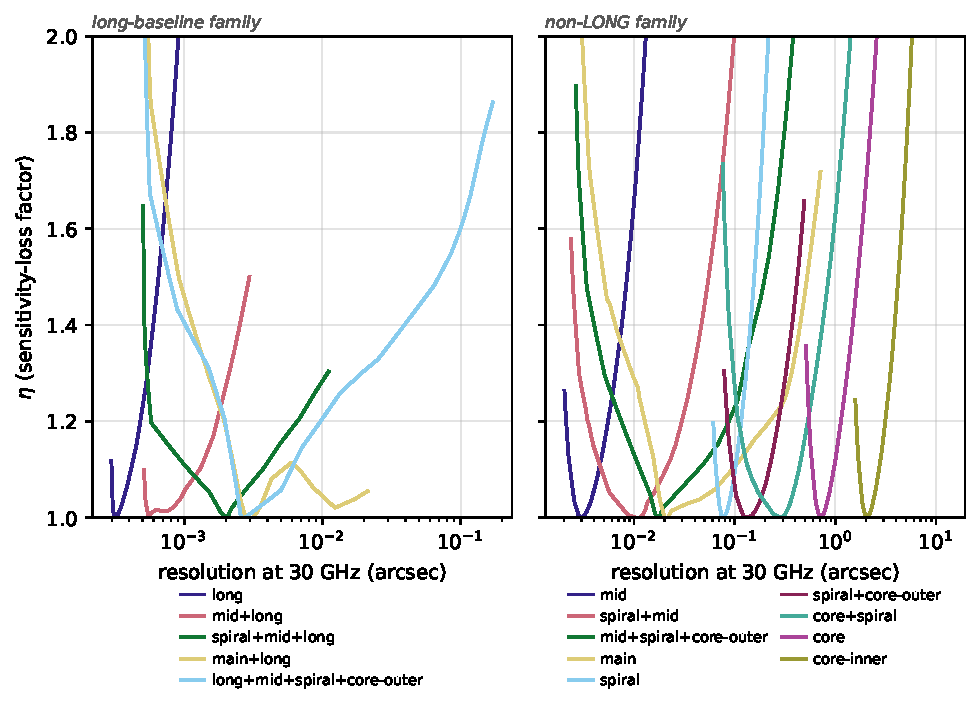
\includegraphics[width=\linewidth]{figs/taperability.pdf}
\caption{Point-source (taperability) curves at 30 GHz: $\eta$ versus
  resolution for the fourteen offered Rev.\,F subarrays, split into
  the LONG-containing family (left) and the non-LONG family (right).
  The panels share a $y$ axis but not an $x$ axis.
  Each curve is the minimum $\eta$ over the $(r,t)$ lattice with no
  constraint on PSF shape.  Heterogeneous subarrays are clipped at
  their beam cap.}
\label{fig:taper}
\end{figure}

\begin{figure}[tbp]
\centering
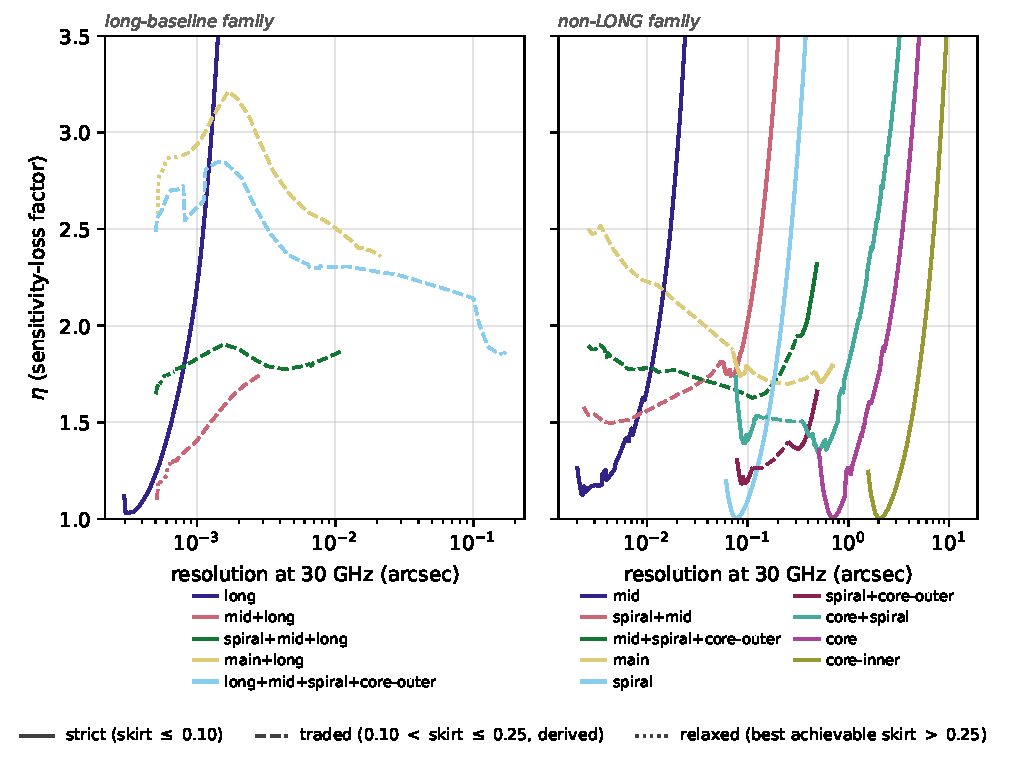
\includegraphics[width=\linewidth]{figs/imaging.pdf}
\caption{Imaging curves at 30 GHz for a 10\% skirt threshold, same
  layout as Figure~\ref{fig:taper}.  Solid segments meet the
  threshold; dashed segments are relaxed points whose best achievable
  skirt lies between 10\% and 25\%; dotted segments have a best
  achievable skirt above 25\%.  The 25\% boundary is a display
  category only and plays no role in the ranking.}
\label{fig:imaging}
\end{figure}

\clearpage

\section{Discussion}
\label{sec:discussion}

We have presented a subarray ranking and selection heuristic that is
consistent with the subarraying concept described in
\cite{saNarrative}, and which further develops methods described in
\cite{memo106}, \cite{memo121}, and references therein.  We also
developed and describe here prototype web and python calculators that
implement these heuristics. These are suitable tools for updating and
refining aspects of the ngVLA design that depend on subarray
selection--- the Envelope Observing Program and its associated size of
compute, for example. They are also suitable tools for beginning to
prototype scheduling heuristics.

Within the context of the approach used here, and generally in ngVLA
imaging studies to date, areas where this prototype could be
improved include:
\begin{enumerate}
\item Improvements to the machinery, e.g., using performance curves
  for the python calculator as well as the web calculator.
\item Measuring the LAS coefficients $C_i$ and their potential
  dependence on $r$ and $t$.
\item Accounting for target declination.
\item Adding additional subarrays, including the SBA; north-south extended options;
  inner- and outer-half mid combinations to fill gaps in the resolution
  curves; inner- and outer-half spiral combinations for the same reason;
  and inward projections of Spiral (spiral+5 and +10) to more efficiently
  cover spiral cases that need modestly improved LAS coverage. 
\item Adding support for continuum (multi-frequency synthesis) cases.
  While this would in principle improve the sculptability of the PSF's
  it would also break the simple frequency re-scaling approach used
  here.  That in turn would require quantifying the impact of the
  approximation (at a minimum),  parameterizing the
  dependence of the performance curves on fractional bandwidth, or implementing some
  other workaround.
\item Parameterizing the impact of varying the field of view, including mosaic
  observations.    
\item Parameterizing the dependence of the performance curves on track length,
  and potentially coupling track length to the calculated integration time.
\end{enumerate}
Taken together, items 5 - 7 in particular point to a large parameter
space with significant complexity and compute cost--- not in
fundamental terms but practically speaking, with current tools, for
the simulations and imaging behind the SA calculator.

As noted by \citep{memo78}, the overall approach of modifying the
synthesized beam's characteristics with $uv$-density based weights
breaks down when too many visibilities occupies their own
$uv$-cell. This regime can occur with short observations (snapshots),
large fields of view, extended arrays, and small numbers of channels
(e.g. cube imaging or MFS with narrow fractional bandwidths). This
fact--- plus the complexity implied by items $5$-$7$ above and the
considerable sensitivity penalty that imaging cases typically pay---
indicate that {\it improved, practical methods of imaging ngVLA data
  are urgently required}.  It is possible, but as yet un-demonstrated,
that it would be sufficient to simply modify the weighting schemes
used by clean--- e.g. an inner $uv$-taper, as proposed on {\tt
  CASR-722}, and/or an adapted form of {\tt briggsbwtaper},
potentially with separate imaging of complementary array components
that get combined later. Advances in interferometric imaging
algorithms in recent decades also provide other options, such as
RESOLVE \citep{resolve} and MPOL \citep{mpol}. Investigations on this
topic should aim to demonstrate stable reconstruction of a variety of
sky images while minimizing loss of sensitivity, and minimizing the
dependence of quantities that need to be measured an tracked on the
specific observing scenario (field of view, track length, number of
channels, etc.).

While changes to the imaging approach would imply changes in the
details of imaging, some metadata, and report content, we consider
that most or all elements of the concept presented here
(Fig.~\ref{fig:arch}) could still be used with appropriate
adaptations.

Finally, in order to provide a clear and fair optimization target for
subarray and imaging heuristics development, it will in the future be
useful to define a representative (priveleged) science product for
each processing block. For example, a specific spectral cube at a
given spectral resolution; the aggregate continuum image; etc.  This
capability should be flexible and PI-driven, with clear
programmatically determinable defaults, and sould not preclude the
generation of other products. It was imlicit in the Subarray
Conceptual Narrative \citep{saNarrative}, but is not yet clearly
stated or defined in detail.

{\it The authors acknowledge the Texas Advanced Computing Center
  (TACC) at The University of Texas at Austin for providing
  computational resources under award AST25010 that have contributed
  to the research results reported within this paper. URL:
  \url{http://www.tacc.utexas.edu}}


\begin{thebibliography}{}

\bibitem{briggs}
Briggs, D.~S. 1995, {\it High Fidelity Deconvolution of Moderately
Resolved Sources}, PhD thesis, New Mexico Institute of Mining and
Technology.

\bibitem{memo96}
Butler, B.~J., Grammer, W., \& Lehmensiek, R. 2021, {\it \ngvla\
Antenna Noise Temperature Calculation}, \ngvla\ Memo 96.

\bibitem{configDescription}
Carilli, C.~L. 2022, {\it Array Configuration: Design Description},
\ngvla\ document 020.23.00.00.00-0002-DSN.

\bibitem{memo78}
Carilli, C.~L., et al. 2020, {\it High Resolution, Wide Field, Narrow
Band, Snapshot Imaging}, \ngvla\ Memo 78.

\bibitem{clark}
Clark, B.~G. 1980, A\&A, 89, 377.

\bibitem{condon2012}
Condon, J.~J., Cotton, W.~D., Fomalont, E.~B., et al.\ 2012, ApJ, 758, 23,
``Resolving the Radio Source Background: Deeper Understanding through Confusion.''
  
\bibitem{mpol}
Czekala, I. et al. 2025, arXiv:2502.00100
  
\bibitem{hogbom}
H{\"o}gbom, J.~A. 1974, A\&AS, 15, 417.

\bibitem{resolve}
Junklewitz, H. et al. 2016, A\&A 586, A76  

\bibitem{memo67}
Mason, B. 2021, {\it Demonstration \& Analysis of \ngvla\ Core + Short
Baseline Array Extended Structure Imaging}, \ngvla\ Memo 67 (v3b).

\bibitem{saNarrative}
Mason, B. et al. 2024, {\it \ngvla\ Subarraying Operational Concept}, \ngvla\
document 020.10.05.05.00-0014-PLA, version A.

\bibitem{matthews2021}
Matthews, A.~M., Condon, J.~J., Cotton, W.~D., \& Mauch, T. 2021, ApJ, 909, 193,
 ``Source Counts Spanning Eight Decades of Flux Density at 1.4 GHz.''

\bibitem{memo55}
Rosero, V. 2019, {\it Taperability Study for the \ngvla\ and
Performance Estimates}, \ngvla\ Memo 55.

\bibitem{memo65}
Rosero, V. 2019, {\it Sculpting of the Synthesized Beam and Image
Fidelity Study of KSG 1: Imaging of Protoplanetary Disks}, \ngvla\
Memo 65.

\bibitem{memo72}
Rosero, V. 2020, {\it A Study of \ngvla\ Subarray Efficiency: Plains +
Fractions of the Core}, \ngvla\ Memo 72.

\bibitem{memo76}
Rosero, V. 2020, {\it Subarray Selection for the Reference Observing
Program}, \ngvla\ Memo 76.

%\bibitem{sensCalc}
%Rosero, V. 2024, {\it \ngvla\ Sensitivity Calculator} (Python),
%\url{https://ngvla.nrao.edu/page/performance}.

\bibitem{memo106}
Rosero, V., \& Carilli, C.~L. 2022, {\it \ngvla\ Imaging Science
Performance Reference Document}, \ngvla\ Memo 106.

\bibitem{memo121}
Rosero, V., \& Mason, B. 2024, {\it Subarray Study for the Envelope
Observing Program}, \ngvla\ Memo 121.

\bibitem{schwab}
Schwab, F.~R. 1984, AJ, 89, 1076.

\end{thebibliography}

\appendix

\section{User's Guide}
\label{sec:guide}

The calculator is the {\tt sa\_select} Python package in the project
repository.  At query time it needs numpy and scipy but not CASA, which is needed
only to regenerate the curves.  The curve tables are shipped with the package as CSV files
({\tt sa\_select/data/}): one row per measured lattice point, with
the subarray name, resolution at 30 GHz, $\eta$, skirt, weighting,
robust, taper, and provenance.

To build a request and rank the subarrays using the Python calculator:
\begin{verbatim}
from sa_select import ObservingRequest, select_subarrays, CurveLibrary

request = ObservingRequest(
    resolution=0.005,       # arcsec (geometric-mean FWHM)
    frequency=30.0,         # GHz
    sensitivity=1e-6,       # Jy/beam (optional; or K)
    las=1.0,                # arcsec (optional)
    imaging=True,           # False = point source
    skirt_threshold=0.10,   # imaging mode only
    beam_margin=0.05)       # fractional beam tolerance

library = CurveLibrary.for_config("revF", "track")
result = select_subarrays(request, library=library)
print(result.table())       # human-readable ranking
rows = result.to_rows()     # list of dicts, one per candidate
best = result.best          # top-ranked feasible candidate
\end{verbatim}
Each feasible candidate carries the achieved beam, $\eta$, the {\tt
tclean} weighting ({\tt weighting}, {\tt robust}, {\tt taper};
{\tt tclean\_pars()} returns them as a {\tt tclean} keyword
dictionary), the
skirt and whether it is relaxed, the subarray LAS at the requested
frequency, the integration time and antenna hours, and any warnings.
Infeasible subarrays are kept in {\tt result.infeasible} with their
exclusion reasons.  The ranking heuristic is selected with {\tt
heuristic=}: a built-in name ({\tt "antenna\_hours"}, the default, or
{\tt "integration\_time"}) or any callable taking the candidate list
and the request and returning it re-ordered.

The same engine runs from the command line:
\begin{verbatim}
python3 -m sa_select --resolution 0.005 --frequency 30 \
    --sensitivity 1e-6 --las 1.0 --imaging --skirt-threshold 0.10
python3 -m sa_select --resolution 0.005 --frequency 30 --point-source
\end{verbatim}
{\tt --rev} and {\tt --sim-mode} select any other registered set of
curves (e.g.\ Rev.\,D track).  Command line invocation reproduces an
EOP-style case list: a CSV with one request per row (columns {\tt
  case, resolution, frequency, sensitivity, sensitivity\_unit, las,
  imaging, beam\_margin, skirt\_threshold, strict\_first, optimize,
  delta\_v}; empty cells fall back to the command-line flags) yields
one output row per case per ranked candidate:
\begin{verbatim}
python3 -m sa_select --batch cases.csv --top 3
\end{verbatim}

An interactive HTML report of all curves, with per-subarray
$(r,t)$ heat maps, is generated by {\tt curvegen/make\_report.py};
Figures~\ref{fig:taper} and \ref{fig:imaging} are drawn by {\tt
memo/figs/make\_figs.py} from the same engine and data.

\section{Regenerating the Curves}
\label{sec:regen}

The simulation and refinement chain is the {\tt curvegen} package,
run under CASA 6 (the {\tt casapy} wrapper) with Slurm on TACC
Stampede3; {\tt docs/ops/RUN\_CAMPAIGNS.md} in the repository is the
full run sheet.  A campaign (one array revision and one simulation
mode) is submitted as a three-stage chain--- simulate, sweep the
lattice, collect--- followed by a PSF-metric backfill:
\begin{verbatim}
bash curvegen/submit_campaign.sh revF track --time 47:00:00
sbatch --array=<combo> --dependency=afterok:<collect_id> \
       curvegen/backfill_psf.sbatch
\end{verbatim}
Here {\tt <combo>} is the campaign index: 0 = Rev.\,F track, 1 =
Rev.\,F snapshot, 2 = Rev.\,D track, 3 = Rev.\,D snapshot, 4 =
Rev.\,C.01 track.  Every stage is resumable: re-running the same command executes only
the missing work.  Measurement sets persist under {\tt \$WORK} and
{\tt tclean} scratch under {\tt \$SCRATCH}.  Refinement rounds are
added to an existing campaign with {\tt
curvegen/adaptive\_retrofit.sbatch}, after which collect, report,
and figure generation are re-run.  The unit tests run from the
repository root with
\begin{verbatim}
casapy -m unittest discover -s tests -t .
\end{verbatim}

\end{document}
